% !TeX spellcheck = en_GB

\pdfbookmark[1]{Super Learner}{sl}

\begin{frame}{Super Learner flow diagram}

\vspace*{0.25em}%
\begin{tikzpicture}
	\tikzset{help lines/.append style=pink}
%	\draw [help lines] (-5,-4) grid (6,4); \node[draw,circle,red] at (0,0) {};
	
	% start with full training data
	\node[right,font=\small] (data) at (-5,0) {$\mathcal{D}=\set{(x_i,y_i)}_1^N$};
	
	% path 1: full training data
	\node[draw,rectangle,minimum width=2cm,minimum height=0.5cm,font=\small] (full) at (-1,2) {$\hat{\phi}_1, \hat{\phi}_2,\dots,\hat{\phi}_K$};
	\begingroup\linespread{0.9}\node[font=\footnotesize,text centered,text width=2.5cm] at ($(full)+(0,0.8)$) {strong learners on full $\mathcal{D}$, $\hat{\phi}_k(\boldsymbol{X})$};\endgroup
	\begingroup\linespread{0.9}\draw[-latex,bend left,thick] (data.north) to node[font=\footnotesize,above left,text centered,text width=1.5cm] {learners prediction} (full.west);\endgroup
	
	% path 2: cross-validation for weights
	\node[font=\footnotesize,below] (cross) at (0,-1.5) {
		$\begin{array}{cccc|c}
			\hat{\phi}_1 & \hat{\phi}_2 &\dots & \hat{\phi}_K & Y \\
			\hline
			1 & 1 & \dots & 1 & 1 \\
			2 & 2 & \dots & 2 & 2 \\
			\vdots & \vdots & \ddots & \vdots & \vdots \\
			V & V & \dots & V & V
		\end{array}$
	};
	\begingroup\linespread{0.95}\node[font=\footnotesize,text centered,text width=3cm] at ($(cross.north)+(0,0.4)$) {cross-validation $\hat{\phi}_{k,T(\nu)}(\boldsymbol{X}_{V(\nu)})$};\endgroup
	\begingroup\linespread{0.9}\draw[-latex,thick,bend right] (data.south) to node[font=\footnotesize,below left,text centered,text width=1.5cm] {prediction weights} (cross);\endgroup
	
	% end with prediction
	\node[left] (pred) at (6,0) {$\hat{\phi}_{\text{SL}}=\sum_{k=1}^K{\color{mLightGreen}\hat{\alpha}_k}{\color{mLightBrown}\hat{\phi}_k}$};
	\draw[-latex,bend left,thick,mLightBrown] (full.east) to (pred);
	%	\draw[-latex,thick,bend right,mLightGreen] (cross) to node[font=\scriptsize,below right,mDarkTeal] {$\argmin_\alpha\sum_{i=1}^NL(Y_i,m(z_i\rvert\alpha))$} (pred);
	\draw[-latex,thick,bend right,mLightGreen] (cross) to (pred);
	\node[font=\footnotesize] (alph) at (4,3.3) {$\hat{\alpha}=\argmin_\alpha\sum_{i=1}^NL(Y_i,m(z_i\rvert\alpha))$};
	\node[font=\footnotesize] at ($(alph)+(0,-0.55)$) {$m(z\rvert\alpha)=\sum_{k=1}^K\alpha_k\hat{\phi}_{k,T(\nu)}\bigl(\boldsymbol{X}_{V(\nu)}\bigr)$};
\end{tikzpicture}

\end{frame}

% ******************************* %
% ******************************* %

%\begin{frame}[fragile]{Super Learner in practice}
%
%% esecuzione in parallelo specifica per Windows
%% azzardo un po': i coefficienti del super learner potrebbero essere di aiuto nella scelta del modello definitivo
%
%\begin{columns}[T]
%\hspace*{-2em}\begin{column}{0.55\textwidth}
%%\vspace*{1cm}%
%\begin{lstlisting}
%SuperLearner(Y, X,
%  cluster,
%  SL.library£!$\,\alert{\leftarrow}\set{\phi_k}$!£,
%  cvControl=list(
%    V=10,shuffle=FALSE))
%\end{lstlisting}
%
%\vspace{0.5em}What's in the ensemble?
%\begin{itemize}
%	\item Response variable mean $\bar{y}$
%	\item Logistic Regression with $\alpha=\numlist{0;1;0.5}$
%	\item Grown and pruned Decision Tree
%	\item Random Forest
%\end{itemize}
%\end{column}
%\hspace*{-3em}\begin{column}{0.5\textwidth}
%% una sorta di variable importance ma per i pesi degli strong learners
%\begin{tikzpicture}
%	%	\draw[help lines] (0,0) grid (6,6); \node[draw,circle,fill=red] at (0,0) {};
%	\node[immagine] at (0,0) {\includegraphics[width=1.23\columnwidth]{../r-StatsLearn-Exam/src/plots/SL-final-coef}};
%	
%	\node[] (phi) at (0.7,6.4) {$\set{\hat{\phi}_k}$};
%	\node[] (alph) at (2.25,0) {$\hat{\alpha}_k$};
%	\draw[-latex,thick] (phi) -- ++(-90:0.8);
%	\draw[-latex,thick] (alph) -- ++(13:1.1);
%\end{tikzpicture}
%%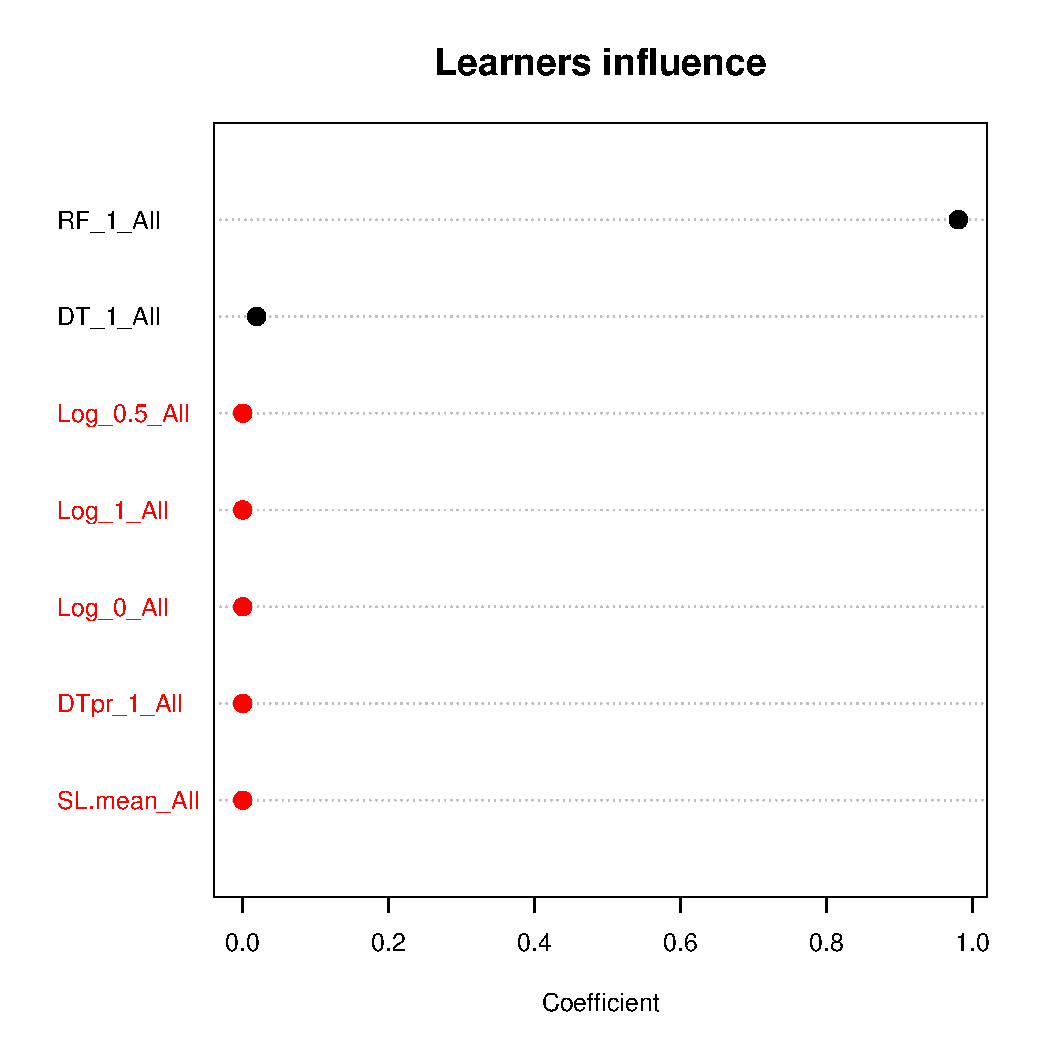
\includegraphics[width=1.23\columnwidth]{../r-StatsLearn-Exam/src/plots/coef-sl-apple}
%\end{column}
%\end{columns}
%
%\end{frame}

% ------------------------------- %

\begin{frame}[fragile]{Super Learner in practice}

% esecuzione in parallelo specifica per Windows
% azzardo un po': i coefficienti del super learner potrebbero essere di aiuto nella scelta del modello definitivo

\begin{columns}[T]
%\hspace*{-2em}
\begin{column}{0.5\textwidth}
%\vspace*{1cm}%
\begin{lstlisting}
SuperLearner(Y, X,
  family=binomial(),
  cluster,
  SL.library£!$\,\alert{\leftarrow}\set{\phi_k}$!£,
  cvControl=list(
    V=10,shuffle=FALSE))
\end{lstlisting}

\begin{lstlisting}
CV.SuperLearner(£!\dots!£)
\end{lstlisting}

% add the code for the library??
\end{column}
%\hspace*{-3em}
\begin{column}{0.5\textwidth}
\vspace{0.5em}What's in the ensemble?
	\begin{itemize}
		\item Response variable mean $\bar{y}$
		\item Logistic Regression with $\alpha=\numlist{0;1;0.5}$
		\item Grown and pruned Decision Tree
		\item Random Forest
		\item Gradient Boosting Machine with $d=1$ and $d=4$
		\item $k\text{NN}$
	\end{itemize}
\end{column}
\end{columns}

\end{frame}

% ******************************* %
% ******************************* %

%\begin{frame}{CV error}
%
%\begin{columns}[T]
%\hspace*{-3.8em}\begin{column}{0.5\textwidth}
%	\includegraphics[width=1.23\columnwidth]{SL-final-coef}
%\end{column}
%\hspace*{-0.5em}\begin{column}{0.5\textwidth}
%	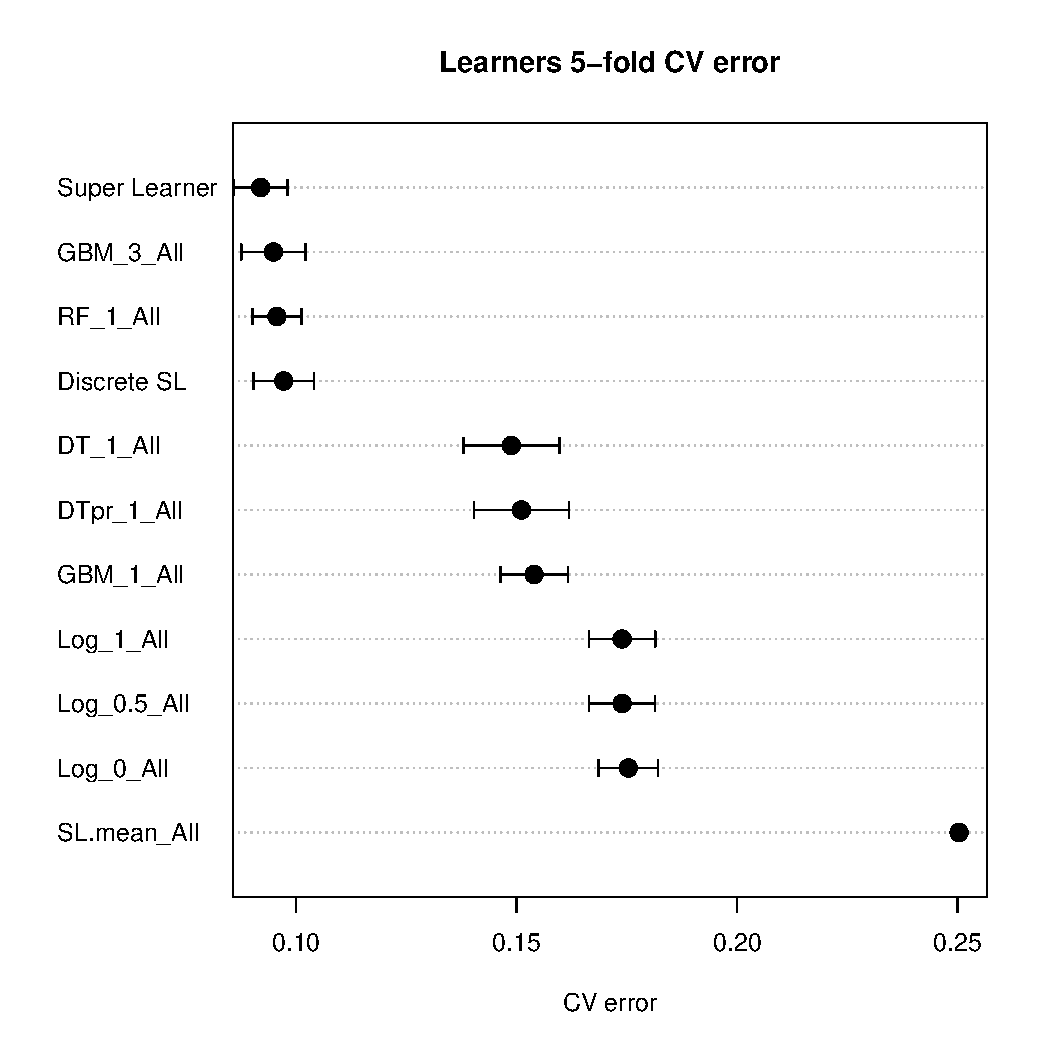
\includegraphics[width=1.2\columnwidth]{SL-final-cv}
%\end{column}
%\end{columns}
%
%\end{frame}
		
\begin{frame}{Super Learner CV error (reduced, w/out $k\text{NN}$)}

\begin{columns}[T]
\hspace*{-4em}%
\begin{column}{0.5\textwidth}
	\begin{tikzpicture}
		%	\draw[help lines] (0,0) grid (6,6); \node[draw,circle,fill=red] at (0,0) {};
		\node[immagine] at (0,0) {\includegraphics[width=1.3\columnwidth]{../r-StatsLearn-Exam/src/plots/SL-final-coef}};
		
		\node[font=\large] (phi) at (0.7,6.7) {$\set{\hat{\phi}_k}$};
		\node[font=\large] (alph) at (2.3,0) {$\hat{\alpha}_k$};
		\draw[-latex,thick] (phi) -- ++(-90:0.8);
		\draw[-latex,thick] (alph) -- ++(13:1.1);
	\end{tikzpicture}
\end{column}
\hspace*{-0.8em}%
\begin{column}{0.5\textwidth}
	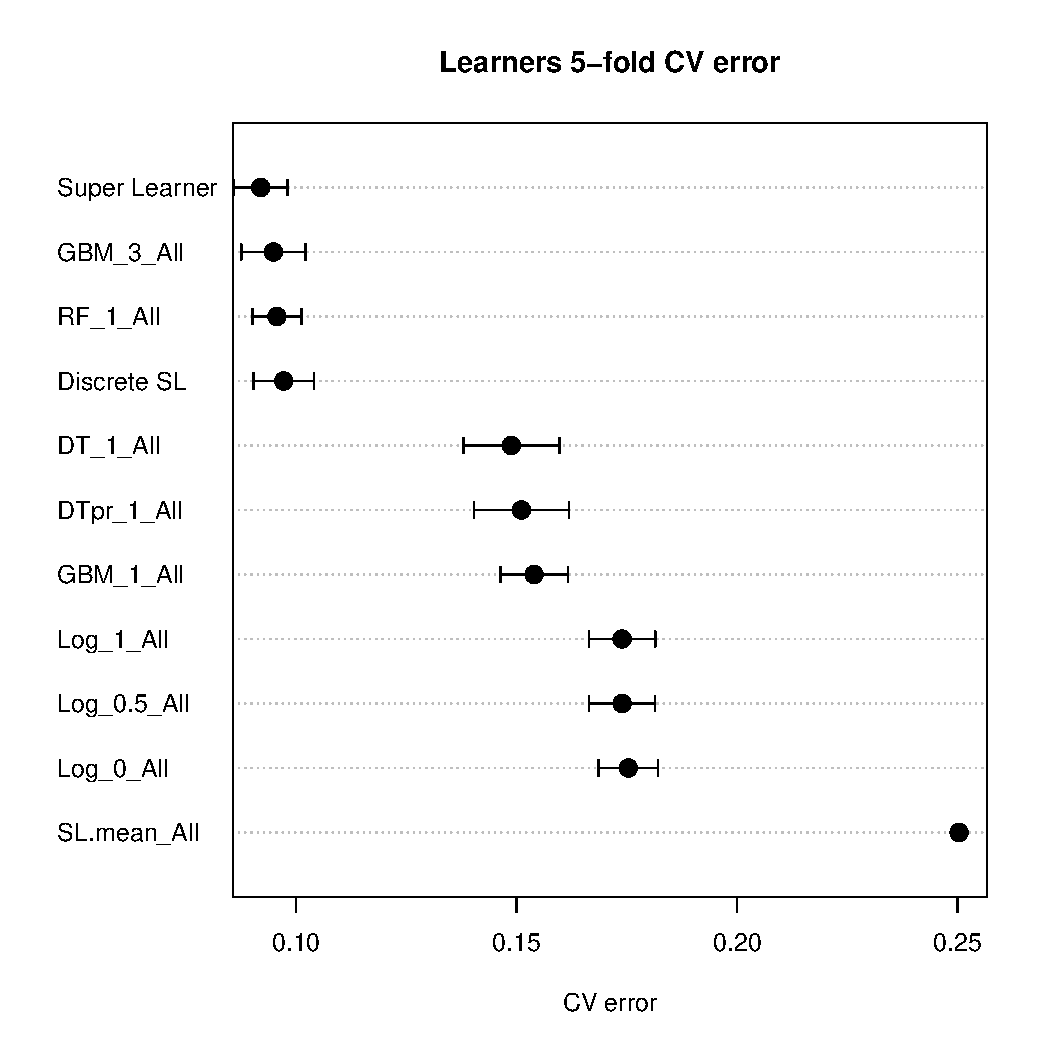
\includegraphics[width=1.3\columnwidth]{SL-final-cv}
\end{column}
\end{columns}

\end{frame}

% ------------------------------- %

\begin{frame}{Super Learner CV error (full)}

\begin{columns}[T]
\hspace*{-4em}%
\begin{column}{0.5\textwidth}
	\begin{tikzpicture}
		%	\draw[help lines] (0,0) grid (6,6); \node[draw,circle,fill=red] at (0,0) {};
		\node[immagine] at (0,0) {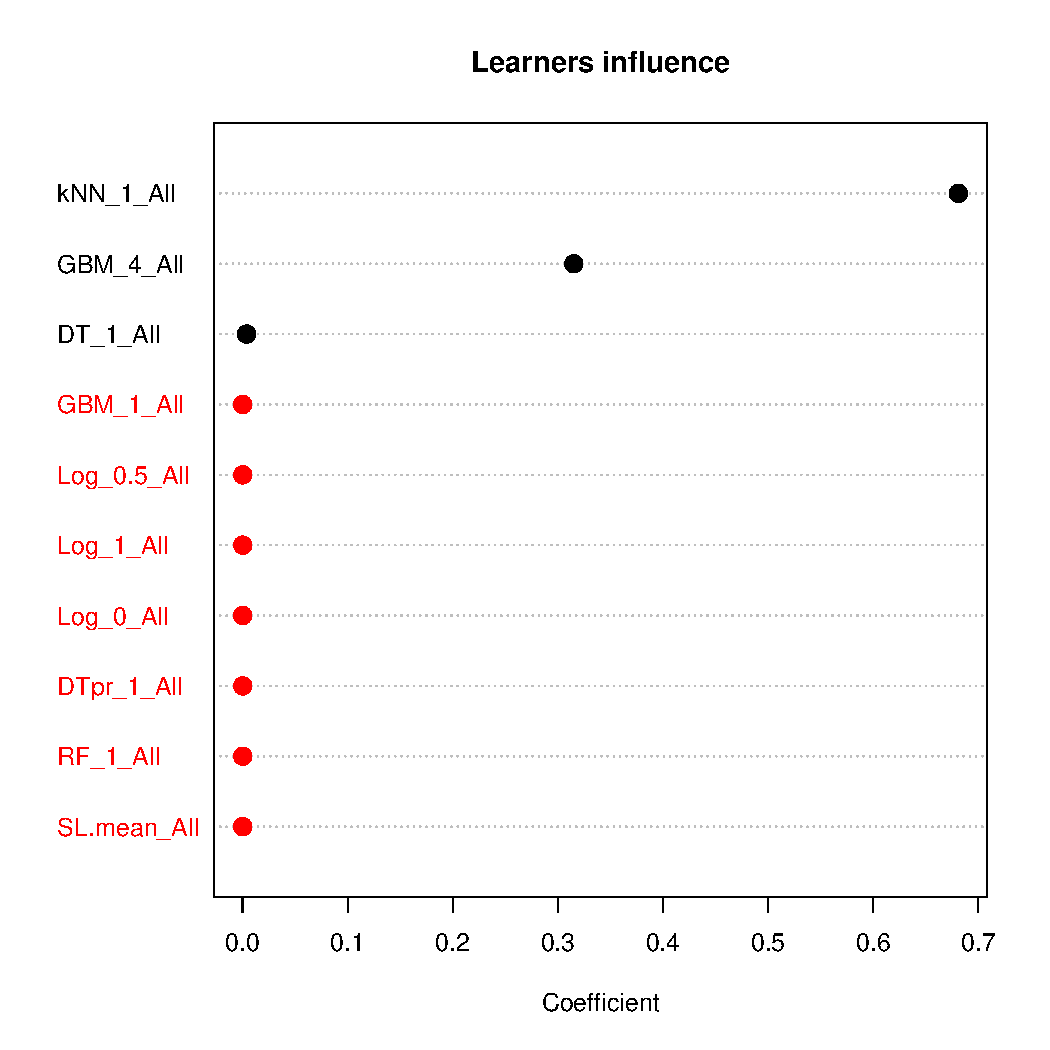
\includegraphics[width=1.3\columnwidth]{../r-StatsLearn-Exam/src/plots/SL-full-coef}};
		
		\node[font=\large] (phi) at (0.7,6.7) {$\set{\hat{\phi}_k}$};
		\node[font=\large] (alph) at (2.3,0) {$\hat{\alpha}_k$};
		\draw[-latex,thick] (phi) -- ++(-90:0.8);
		\draw[-latex,thick] (alph) -- ++(13:1.1);
	\end{tikzpicture}
\end{column}
\hspace*{-0.8em}%
\begin{column}{0.5\textwidth}
	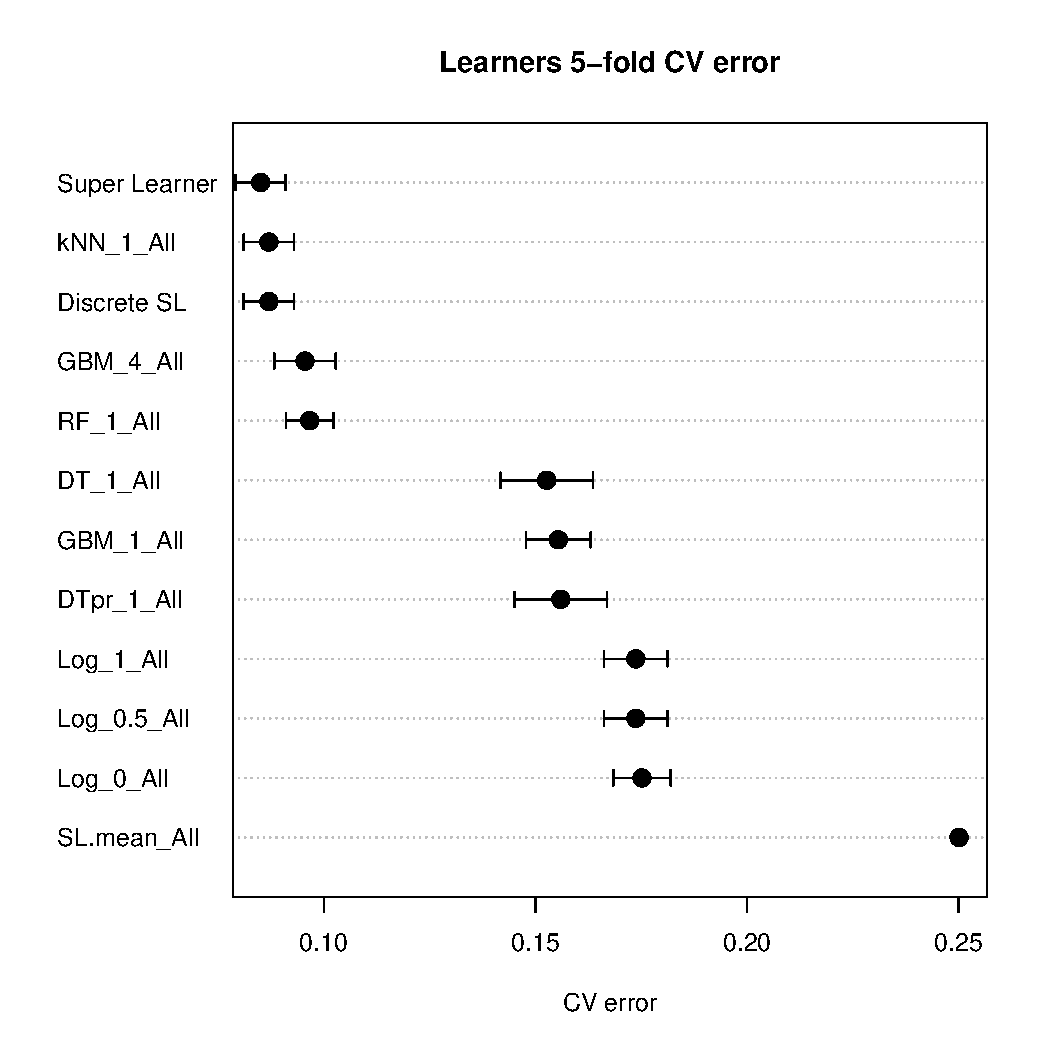
\includegraphics[width=1.3\columnwidth]{SL-full-cv}
\end{column}
\end{columns}

\end{frame}
